\pagestyle{plain}
\graphicspath{{Chapter3/Figs/Raster/}{Chapter3/Figs/}}
% \chapter{Mô hình Boosted Tree cho phát hiện xâm nhập mạng}
\chapter{MÔ HÌNH BOOSTED TREE CHO PHÁT HIỆN XÂM NHẬP MẠNG}
Chương này mô tả cách thiết lập thực nghiệm, đưa ra các mô hình thực  nghiệm, giới thiệu các công cụ được sử dụng trong bài toán, kết quả thực nghiệm và phân tích đánh giá.
\section{Giới thiệu bộ dữ liệu UNSW-NB15}

Một hệ thống phát hiện xâm nhập dựa trên mạng (NIDS)giám sát các luồng dữ liệu để xác định có xuất hiện xâm nhập hay không. Như đã đề cập, NIDS được phân thành 2 loại, signature based - giám sát dựa trên chữ ký và anomaly based - giám sát truy nhập dựa trên bất thường. Signature based sẽ so khớp mỗi traffic flow với một loại tấn công đã biết để phát hiện ra xâm nhập. Ngược lại, với phương pháp Anomaly based, một hồ sơ được tạo ra với các hành vi "bình thường", tất cả các hành vi lệch với hồ sơ đều được coi là tấn công. Các Signature based NIDS sẽ không phát hiện được các loại tấn công chưa biết, do đó việc sử dụng Anomaly based được khuyến nghị.\\
\indent Để đánh giá hiệu quả của NIDS, chúng ta cần một bộ dữ liệu gồm các hành vi bình thường và bất thường. Các bộ dữ liệu như KDDCUP 99 \cite{kdd99} và NSLKDD \cite{nslkdd} được sử dụng rộng rãi để đánh giá hiệu năng của NIDS. Tuy nhiên, qua một vài nghiên cứu \cite{17}\cite{18}\cite{19}\cite{20}, việc đánh giá NIDS qua các bộ dữ liệu này không phản ánh kết quả thực tế vì một số lý do. Thứ nhất, bộ dữ liệu KDD 99 chứa một số lượng lớn các bản ghi thừa trong tập huấn luyện. Các bản ghi dư thừa này ảnh hưởng lớn đến kết quả phát hiện. Thứ hai, trong bộ dữ liệu này thiếu nhiều các bản ghi, điều này làm thay đổi bản chất của dữ liệu. Thứ ba, tuy bộ NSLKDD, một phiên bản cải tiến của KDDCUP 99, đã giải quyết một số vấn đề về mất cân bằng dữ liệu giữa các bản ghi bình thường/bất thường hoặc là các giá trị bị thiếu. Tuy nhiên, bộ dữ liệu này vẫn không phải là một bộ dữ liệu giúp đánh giá toàn diện NIDS trong môi trường tấn công hiện đại.\\
\indent Chính vì các lý do trên, một nhóm nghiên cứu thuộc viện nghiên cứu của Trung tâm An ninh mạng Úc (Australian Centre of Cyber Security - ACCC) và các nhà nghiên cứu về lĩnh vực này trên toàn cầu đã cho ra mắt bộ dữ liệu UNSW-NB15 nhằm giúp ích trong việc đánh giá một NIDS.

\subsection{Phương pháp thu thập dữ liệu}

Công cụ IXIA PerfectStorm\cite{ixia} được sử dụng để tạo ra các traffic bình thường và bất thường. Dữ liệu bất thường đi qua IXIA mô phỏng 9 loại tấn công mô tả trong Bảng 3.1. Công cụ IXIA bao gồm tất cả thông tin về các loại tấn công mới được cập nhật liên tục tại trang CVE\cite{cve}, một bộ từ điển công khai các lỗ hổng bảo mật.\\
Bắt các lưu lượng mạng dưới dạng gói tin bằng cách sử dụng công cụ tcmdump. Việc mô phỏng kéo dài 16 giờ ngày 22/01/2015 và 15 giờ ngày 17/02/2015, thu được 100Gb dữ liệu. Mỗi Pcap file được chia nhỏ mỗi file 1000MB bằng tcpdump. Argus và Bro-IDS được sử dụng để tạo ra các đặc trưng tin cậy. Thêm vào đó, 12 thuật toán được phát triển sử dụng ngôn ngữ C\# để phân tích sâu các gói tin. Bộ dữ liệu được gán nhãn bao gồm tất cả các loại tấn công được mô phỏng. 

\begin{center}

	\begin{figure}[H]
		\includegraphics[scale=0.5]{images/Chap3-Figure1} 
		\caption{Kiến trúc mô hình sinh bộ dữ liệu UNSW-NB15 }
	\end{figure}

\end{center}
\begin{center}
    \begin{table}[H]
    
   	\begin{tabular}{|c|c|c|m{8cm}|}%{|c|c|c|}
        \hline
        \textbf{Loại} & \textbf{Số lượng bản ghi} & \textbf{Tỉ lệ} &\textbf{Mô tả}\\
        \hline
        Normal & 1,765,693 & 84.6\% & Dữ liệu tương tác bình thường\\
        \hline
        Fuzzers & 24,246 & 1.16\% & Cố gắng khiến một chương trình hoặc hệ thống mạng bị đình chỉ bằng cách sinh dữ liệu ngẫu nhiên\\
        \hline
        Analysis & 2,677 & 0.12\% & Bao gồm nhiều loại tấn công khác nhau: quét cổng, spam và xâm nhập các file html\\
        \hline
        Backdoors & 2,329 & 0.11\% & Một kỹ thuật vượt qua hệ thống xác thực để truy nhập vào máy tính hoặc dữ liệu\\
        \hline
        DoS & 16,353 & 0.78\% &Tấn công từ chối dịch vụ\\
        \hline
        Exploits & 44,525 & 2.13\% &Hacker khai thác lỗ hổng bảo mật đã biết trước của hệ thống\\
        \hline
        Generic & 215,481 & 10.32\% & Kỹ thuật chống lại mã hóa khối.\\
        \hline
        Reconnaissance & 13,987 & 0.67\% & Bao gồm tất cả Strikes mô phỏng lại việc thu thập thông tin\\
        \hline
        Shellcode & 1,511 & 0.07\% & Một đoạn code ngắn được sử dụng như payload trong khai thác lỗ hổng phần mềm\\
        \hline
        Worms & 174 & 0.008\% &Các tập tin độc hại tự nhân bản để lan sang các máy tính khác.\\
        \hline
    \end{tabular}
    \caption{Phân bố bản ghi của bộ dữ liệu}
    \end{table}
\end{center}
\vspace{1cm}

\def\angle{0}
\def\radius{3}
\def\cyclelist{{"orange","blue","red","green"}}
\newcount\cyclecount \cyclecount=-1
\newcount\ind \ind=-1
    \begin{figure}[H]
        \centering
        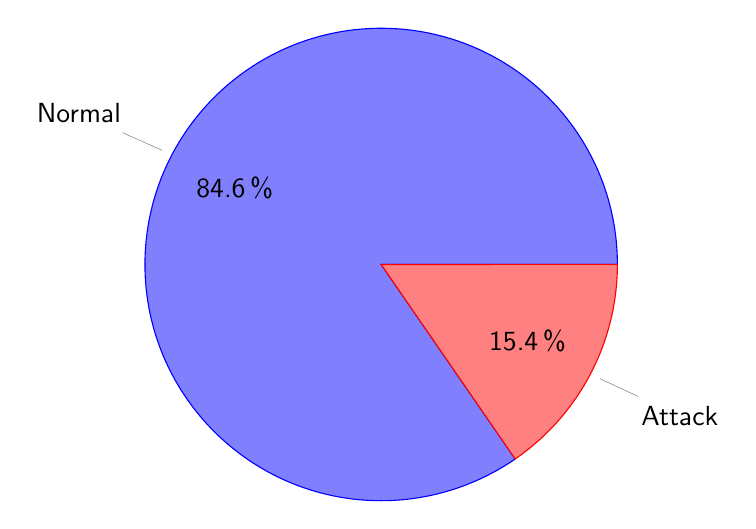
\begin{tikzpicture}[nodes = {font=\sffamily}]
      \foreach \percent/\name in {
          84.6/Normal,
          15.4/Attack
        } {
          \ifx\percent\empty\else               % If \percent is empty, do nothing
            \global\advance\cyclecount by 1     % Advance cyclecount
            \global\advance\ind by 1            % Advance list index
            \ifnum3<\cyclecount                 % If cyclecount is larger than list
              \global\cyclecount=0              %   reset cyclecount and
              \global\ind=0                     %   reset list index
            \fi
            \pgfmathparse{\cyclelist[\the\ind]} % Get color from cycle list
            \edef\color{\pgfmathresult}         %   and store as \color
            % Draw angle and set labels
            \draw[fill={\color!50},draw={\color}] (0,0) -- (\angle:\radius)
              arc (\angle:\angle+\percent*3.6:\radius) -- cycle;
            \node at (\angle+0.5*\percent*3.6:0.7*\radius) {\percent\,\%};
            \node[pin=\angle+0.5*\percent*3.6:\name]
              at (\angle+0.5*\percent*3.6:\radius) {};
            \pgfmathparse{\angle+\percent*3.6}  % Advance angle
            \xdef\angle{\pgfmathresult}         %   and store in \angle
          \fi
        };
    \end{tikzpicture}
    \caption{Tỉ lệ nhãn bình thường và nhãn tấn công}
\end{figure}

\newcount\ind \ind=-1
    \begin{figure}[H]
        \centering
        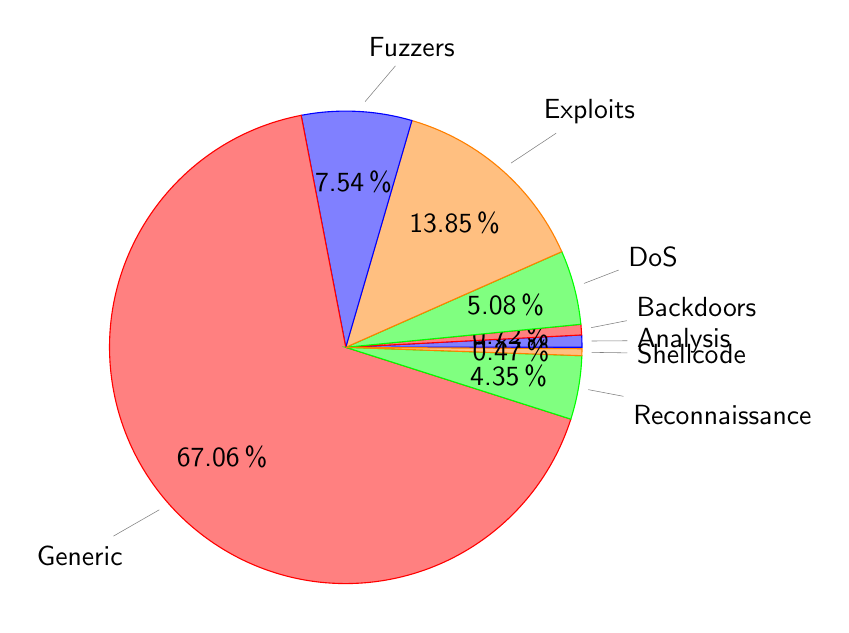
\begin{tikzpicture}[nodes = {font=\sffamily}]
      \foreach \percent/\name in {
          0.83/Analysis,
          0.72/Backdoors,
          5.08/DoS,
          13.85/Exploits,
          7.54/Fuzzers,
          67.06/Generic,
          4.35/Reconnaissance,
          0.47/Shellcode,
          /Worms
        } {
          \ifx\percent\empty\else               % If \percent is empty, do nothing
            \global\advance\cyclecount by 1     % Advance cyclecount
            \global\advance\ind by 1            % Advance list index
            \ifnum3<\cyclecount                 % If cyclecount is larger than list
              \global\cyclecount=0              %   reset cyclecount and
              \global\ind=0                     %   reset list index
            \fi
            \pgfmathparse{\cyclelist[\the\ind]} % Get color from cycle list
            \edef\color{\pgfmathresult}         %   and store as \color
            % Draw angle and set labels
            \draw[fill={\color!50},draw={\color}] (0,0) -- (\angle:\radius)
              arc (\angle:\angle+\percent*3.6:\radius) -- cycle;
            \node at (\angle+0.5*\percent*3.6:0.7*\radius) {\percent\,\%};
            \node[pin=\angle+0.5*\percent*3.6:\name]
              at (\angle+0.5*\percent*3.6:\radius) {};
            \pgfmathparse{\angle+\percent*3.6}  % Advance angle
            \xdef\angle{\pgfmathresult}         %   and store in \angle
          \fi
        };
    \end{tikzpicture}
    \caption{Tỉ lệ nhãn từng nhãn tấn công trong tổng các số nhãn tấn công}
\end{figure}

\subsection{Cấu hình cho IXIA}
Theo hình 3.1, bộ sinh lưu lượng IXIA được cấu hình với 3 server ảo. Server 1 và 3 được cấu hình để sinh ra các lưu lượng mạng bình thường còn server được dùng để sinh các lưu lượng mạng bất thường. Thiết lập kết nối giữa các server để thu được các lưu lượng riêng tư và công khai, có 2 virtual interface với IP 10.40.85.30 và 10.40.184.30. Các server được kết nối tới các host qua các router. Router 1 có IP 10.40.184.30 và 10.40.85.30, router 2 có IP 10.40.184.1 và 10.40.183.1. Các router kết nối tới tường lửa đã được cấu hình để cho tất cả các lưu lượng mạng đi qua. Công cụ tcpdump được cài đặt tại router 1 để bắt các Pcap file trong khi mô phỏng. Ý đồ chính của việc này nhằm để bắt các lưu lượng bình thường và bất thường, bắt nguồn từ công cụ IXIA và phân tán trong các nút mạng. Điều quan trọng là công cụ IXIA được sử dụng như một bộ sinh lưu lượng tấn công với các hành vi từ CVE nhằm mô phỏng chính xác nhất môi trường tấn công hiện đại. Dựa vào tốc độ lưu lượng mạng và phương pháp khai thác của các kiểu tấn công hiện đại, công cụ IXIA sinh ra 1 cuộc tấn công mỗi giây trong thời gian mô phỏng, thu về 50 GB đầu. Với cách mô phỏng và cấu hình thứ 2 sinh ra được 10 cuộc tấn công mỗi giây, thu được 50 GB còn lại.

\subsection{Danh sách các đặc trưng trong bộ dữ liệu}
\begin{figure}[H]
		\includegraphics[scale=0.5]{images/Chap3-Figure1} 
		\caption{Minh họa mô hình tạo bộ dữ liệu UNSW-NB15}
\end{figure}
Bộ dữ liệu được tạo ra theo mô hình như Hình 3.2. Các đặc trưng trong các file csv được chia thành các nhóm chính như sau:

Các đặc trưng mô tả luồng kết nối:

\begin{table}[H]
    \centering
    \begin{tabular}{|c|c|c|l|}
        \hline
        \textbf{\#}  & \textbf{Tên} & \textbf{T} & \textbf{Mô tả} \\
        \hline
        1 & \textit{scrip} & N & Địa chỉ IP nguồn \\
        \hline
        2 & \textit{sport} & I & Port nguồn\\
        \hline
        3 & \textit{dstip} & N & Địa chỉ IP đích \\
        \hline
        4 & \textit{dstport} & I & Port đích \\
        \hline
        5 & \textit{proto} & N & Giao thức \\
        \hline
    \end{tabular}
    \caption{Đặc trưng luồng}
    
\end{table}

Các đặc trưng thu được từ bộ công cụ Argus và Bro-IDS. Các đặc trưng này bao gồm các đặc trưng dựa trên gói tin (packet-based) và các đặc trưng dựa trên lưu lượng (flow-based). Các đặc trưng dựa trên gói tin hỗ trợ kiểm tra payload bên cạnh tiêu đề (header) của các gói. Ngược lại, để thu được đặc trưng dựa trên luồng và duy trì phân tích tính toán với chi phí thấp thay vì quan sát tất cả các gói tin đi qua mạng, chỉ các gói kết nối tới mạng được xem xét. Các đặc trưng được phân thành ba nhóm: Cơ bản, Nội dung và Thời gian được mô tả trong các Bảng 3.3, 3.4 và 3.5.

\begin{table}[H]
    \centering
    \begin{tabular}{|c|c|c|l|}
        \hline
        \textbf{\#}  & \textbf{Tên} & \textbf{T} & \textbf{Mô tả} \\
        \hline
        6 & \textit{state} & N & Trạng thái phụ thuộc vào giao thức \\
        \hline
        7 & \textit{dur} & F & Thời gian thu thập của bản ghi\\
        \hline
        8 & \textit{sbytes} & I & Số byte từ nguồn đến đích\\
        \hline
        9 & \textit{dbytes} & I & Số byte từ đích đến nguồn \\
        \hline
        10 & \textit{sttl} & I &  Thời gian sống từ nguồn đến đích\\
        \hline
        11 & \textit{dttl} & I &  Thời gian sống từ đích đến nguồn\\
        \hline
        12 & \textit{sloss} & I &  Các gói nguồn được truyền lại hoặc bị rớt\\
        \hline
        13 & \textit{dloss} & I &  Các gói đích được truyền lại hoặc bị rớt\\
        \hline
        14 & \textit{service} & N & http, ftp, ssh, dns ..,hoặc (-) \\
        \hline
        15 & \textit{sload} & F & Số bit nguồn trong một giây \\
        \hline
        16 & \textit{dload} & F &  Số bit đích trong một giây\\
        \hline
        17 & \textit{spkts} & I &  Số packet từ nguồn đến đích\\
        \hline
        18 & \textit{dpkts} & I &  Số packet từ đích về nguồn\\
        \hline
    \end{tabular}
    \caption{Các đặc trưng cơ bản}
    
\end{table}

\begin{table}[H]
    \centering
    \begin{tabular}{|c|c|c|l|}
        \hline
        \textbf{\#}  & \textbf{Tên} & \textbf{T} & \textbf{Mô tả} \\
        \hline
        19 & \textit{swin} & I & Cửa sổ TCP nguồn\\
        \hline
        20 & \textit{dwin} & I & Cửa sổ TCP đích\\
        \hline
        21 & \textit{stcpb} & I & Số thứ tự TCP nguồn\\
        \hline
        22 & \textit{dtcpb} & I & Số thứ tự TCP đích\\
        \hline
        23 & \textit{smeansz} & I & Kích thức trung bình của luồng truyền qua nguồn\\
        \hline
        24 & \textit{dmeansz} & I & Kích thước trung bình của luồng truyền qua đích\\
        \hline
        25 & \textit{trans\_depth} & I & Độ sâu kết nối của http request/response\\
        \hline
        26 & \textit{res\_bdy\_len} & I & Kích thức nội dung truyền từ máy chủ http \\
        \hline
    \end{tabular}
    \caption{Các đặc trưng nội dung}
    
\end{table}

\begin{table}[H]
    \centering
    \begin{tabular}{|c|c|c|l|}
        \hline
        \textbf{\#}  & \textbf{Tên} & \textbf{T} & \textbf{Mô tả} \\
        \hline
        27 & \textit{sjit} & F & jitter nguồn\\
        \hline
        28 & \textit{djit} & F & jitter đích\\
        \hline
        29 & \textit{stime} & T & Thời gian bắt đầu ghi\\
        \hline
        30 & \textit{ltime} & T & Thời gian kết thúc ghi\\
        \hline
        31 & \textit{sintpkt} & F & Thời gian đến gói tin giữa các gói tin nguồn(mSec)\\
        \hline
        32 & \textit{dintpkt} & F & Thời gian đến gói tin giữa các gói tin đích (mSec)\\
        \hline
        33 & \textit{tcprtt} & F &  Tổng số 'synack' và 'ackdat' của TCP\\
        \hline
        34 & \textit{synack} & F &  Thời gian giữa gói tin SYN và SYN\_ACK\\
        \hline
        35 & \textit{ackdat} & F &  Thời gian giữa gói tin SYN\_ACK và ACK \\
        \hline
    \end{tabular}
    \caption{Đặc trưng thời gian}
    
\end{table}
Bảng 3.6 mô tả về các đặc trưng bổ sung của bộ dữ liệu UNSW-NB15. Các đặc trưng từ 36-40 là các đặc trưng mục đích chung, các đặc trưng 41-47 là các đặc trưng của kết nối. Với đặc trưng mục đích chung, mỗi tính năng có mục đích riêng, theo quan điểm phòng thủ, trong khi đó các đặc trưng kết nối chỉ được tạo ra để cung cấp biện pháp phòng vệ trong trong các kịch bản kết nối. Những kẻ tấn công có thể quét máy chủ theo cách tự lập. Ví dụ, mỗi lần một phút hoặc một lần quét trên một giờ. Để xác định những kẻ tấn công này, các đặc trưng 36-47 của Bảng 3.6 được sắp xếp theo thứ tự tương ứng với đặc trưng cuối cùng để thu thập các đặc tính tương tự của các bản ghi kết nối với 100 kết nối tuần tự.

\begin{table}[H]
    \centering
    \begin{tabular}{|c|c|c|m{8cm}|}
        \hline
        \textbf{\#}  & \textbf{Tên} & \textbf{T} & \textbf{Mô tả} \\
        \hline
        36 & \textit{is\_sm\_ips\_ports} & B & Nếu nguồn và đích cùng ip và port thì là 1, ngược lại là 0 \\
        \hline
        37 & \textit{ct\_state\_ttl} & I & Số lượng mỗi trạng thái (6) theo phạm vi giá trị cụ thể của thời gian sống nguồn / đích\\
        \hline
        38 & \textit{ct\_flw\_http\_mthd} & I & Số lượng luồng dùng phương thức POST và GET trong http\\
        \hline
        39 & \textit{is\_ftp\_login} & B & 1 nếu dịch vụ ftp được truy cập bởi user, ngược lại là 0\\
        \hline
        40 & \textit{ct\_ftp\_cmd} & B & Số lượng luồng có 1 lệnh trong phiên ftp\\
        \hline
        41 & \textit{ct\_srv\_src} & I & Số lượng kết nối dùng cùng một dịch vụ và địa chỉ nguồn(1) trong 100 kết nối theo (26)\\
        \hline
        42 & \textit{ct\_srv\_dst} & I & Số lượng kết nối dùng cùng một dịch vụ và địa chỉ đích(1) trong 100 kết nối theo (26) \\
        \hline
        43 & \textit{ct\_dst\_ltm} & I &  Số lượng kết nối có cùng đích trong 100 kết nối theo (26)\\
        \hline
        44 & \textit{ct\_src\_ ltm} & I & Số lượng kết nối có cùng địa chỉ nguồn trong 100 kết nối theo (26) \\
        \hline
        45 & \textit{ct\_src\_dport\_ltm} & I &  Số lượng kết nối có cùng địa chỉ nguồn (1) và cổng đích (4) trong 100 kết nối theo (26)\\
        \hline
        46 & \textit{ct\_dst\_sport\_ltm} & I &  Số lượng kết nối có cùng địa chỉ đích (3) và cổng nguồn (2) trong 100 kết nối theo (26)\\
        \hline
        47 & \textit{ct\_dst\_src\_ltm} & I & Số lượng kết nối có cùng địa chỉ nguồn và đích trong 100 kết nối theo (26) \\
        \hline
    \end{tabular}
    \caption{Đặc trưng bổ sung}
    
\end{table}

2 đặc trưng cuối cùng trong bộ dữ liệu là các nhãn. 
\begin{table}[H]
    \centering
    \begin{tabular}{|c|c|c|l|}
        \hline
        \textbf{\#}  & \textbf{Tên} & \textbf{T} & \textbf{Mô tả} \\
        \hline
        48 & \textit{attack\_cat} & N & Tên của các nhãn tấn công, bao gồm 9 nhãn \\
        \hline
        49 & \textit{Label} & B & 1 là tấn công, 0 là bình thường\\
        \hline
    \end{tabular}
    \caption{Các nhãn}
    
\end{table}
\section{Phương pháp đánh giá}
Để đánh giá hiệu quả của mô hình phân loại, đồ án sử dụng phương pháp Ma trận lỗi (Error Matrix hay Confusion matrix \cite{confusion}). Mỗi hàng của ma trận đại diện cho một nhãn được dự đoán, trong khi mỗi cột của ma trận đại diện cho một nhãn chính xác. \\
Từ Ma trận lỗi, chúng ta có thể tính được các giá trị cho mỗi nhãn k trong bộ dữ liệu, bao gồm Độ chính xác(Precision), độ phủ (Recall) và F1 (Trung bình điều hòa): \\
\indent Độ chính xác được định nghĩa là tổng số quan sát có nhãn $c_i$ được dự đoán chính xác chia cho tổng số các quan sát được dự đoán có nhãn $c_i$.
\begin{equation}
P(c_i) = \frac{\text{Số quan sát được gán chính xác nhãn }c_i}{\text{Tổng số quan sát được gán nhãn }c_i}
\end{equation}
\indent Độ phủ được tính bằng tổng số các quan sát có nhãn $c_i$ được dự đoán chính xác chia cho tổng số các quan sát có nhãn $c_i$ trong tập kiểm thử.
\begin{equation}
R(c_i) = \frac{\text{Số quan sát được gán chính xác nhãn }c_i}{\text{Tổng số các quan sát có nhãn $c_i$ trong tập huấn luyện}}
\end{equation}
F1 là một trung bình điều hòa của các tiêu chí P và R. F1 có các tính chất sau: 
\begin{itemize}
\ii F1 có xu hướng lấy giá trị gần với giá trị nào nhỏ hơn giữa 2 giá trị P và R.
\ii F1 có giá trị lớn nếu cả 2 giá trị P và R đều lớn.
\end{itemize}
\begin{equation}
P(c_i) = \frac{2 * P * R}{P + R}
\end{equation}

\section{Thực nghiệm}
\subsection{Hệ thống máy tính}
Cấu hình phần cứng phục vụ cho quá trình huấn luyện:
\begin{itemize}
    \item Vi xử lý: Intel Corporation Xeon E7 v3/Xeon E5 v3/Core i7 Power Control Unit
    \item RAM: 157.0 GB
    \item Hệ điều hành: Ubuntu Server 16.04
    \item Dung lượng ổ cứng 2TB
\end{itemize}
\subsection{Các chương trình và thư viện phần mềm}
\subsubsection*{Pandas}
Pandas là thư viện mã nguồn mở, được cấp phép bởi BSD, cung cấp các cấu trúc dữ liệu hiệu năng cao, dễ sử dụng và các công cụ phân tích dữ liệu cho ngôn ngữ lập trình Python.
Pandas bao gồm:
\begin{itemize}
    \item Tập hợp các cấu trúc dữ liệu dạng mảng, phần chính là Series và DataFrame
    \item Các đối tượng chỉ mục cho phép lập chỉ mục trục đơn giản và lập chỉ mục trục đa cấp / phân cấp
    \item Bộ công cụ tích hợp để chuyển đổi và tập hợp dữ liệu
    \item Bộ sinh dữ liệu theo ngày
    \item Bộ công cụ I/O: Đọc dữ liệu dạng bảng ở các file (CSV, delimited, Excel 2003) và lưu các đối tượng pandas theo PyTables/HDF5 format.
    \item Các phiên lưu trữ dữ liệu thưa trên bộ nhớ hiệu quả, các cấu trúc dữ liệu tiêu chuẩn để lưu trữ dữ liệu thiếu hoặc hằng số (một số có giá trị cố định)
    \item Các cửa sổ thống kê
\end{itemize}

\subsubsection*{Scikit-learn}
Scikit-learn là thư viện mã nguồn mở dùng cho ngôn ngữ lập trình Python. Scikit-learn bao gồm rất nhiều các thuật toán học máy phân cụm, hồi quy, phân loại,.. và được thiết kế để tương thích với các thư viện số học như Numpy \cite{numpy} và SciPy \cite{scipy} 
\subsubsection*{Thư viện XGBoost}
XGBoost\cite{4} là thư viện mã nguồn mở, cài đặt thuật toán Boosted Tree đã mô tả ở chương 2, dùng để áp dụng vào các bài toán học máy. Đây là thư viện mạnh mẽ, đã thống trị học máy ứng dụng và các cuộc thi về Khoa học dữ liệu trên Kaggle\cite{15}trong thời gian gần đây. XGBoost hỗ trợ rất nhiều các giao diện (interface) như:
\begin{itemize}
\ii Giao diện dòng lệnh (CLI - Command line interface).
\ii C++
\ii Python interface cùng với mô hình theo chuẩn Scikit-learn
\ii R interface
\ii Julia
\ii Java và các ngôn ngữ sử dụng JVM như Scala, các platform như Hadoop
\end{itemize}
Đồ án sử dụng Python interface để huấn luyện mô hình.

\section{Tiền xử lý dữ liệu}
\subsection{Loại bỏ các đặc trưng dư thừa}
Như đã mô tả ở phần 3.1.2, UNSW-NB15 là một bộ dữ liệu được tạo ra từ phòng thí nghiệm với số lượng IP cố định. Dựa vào các cuộc xâm nhập mạng trong thực tế, các IP đến từ rất nhiều nguồn và port khác nhau. Việc sử dụng các đặc trưng này sẽ khiến mô hình học bị overfit, khi đưa áp dụng vào thực tế sẽ đưa ra dự đoán thiếu chính xác. Vì vậy, các đặc trưng \ \textit{Srcip}, \textit{Sport}, \textit{Dstip}, \textit{Dport} được loại bỏ khỏi tập dữ liệu.\\
Các đặc trưng \textit{Stime} - thời gian bắt đầu ghi, \textit{Ltime} - thời gian kết thúc ghi được thay thế bằng đặc trưng \textit{duration} - độ dài thời gian ghi dữ liệu.\\
Các đặc trưng nhãn mô tả ở Bảng 3.7 được tách riêng ra.
Bảng 3.8 và 3.9 là ví dụ về việc bỏ các thuộc tính thừa:
\begin{table}[H]
    \centering
    \begin{tabular}{|m{8cm}|}
    \hline
         '59.166.0.4' 17491 '149.171.126.0' '53' 'udp' 'CON' 0.001256 132.0 164.0 31.0 29.0 0.0 0.0 'dns' 420382.15629999997 522293.0 2.0 2.0 0.0 0.0 0.0  0.0 66.0 82.0 0.0 0.0 0.0 0.0 1421927424.0 1421927424.0 0.012 0.0080000000000000002 0.0 0.0 0.0 0.0 0.0 0.0 0.0 0.0 12.0 13.0 1.0 1.0 1.0 1.0 1.0 nan 0.0\\
         \hline
    \end{tabular}
    \caption{Bản ghi trước khi bỏ các đặc trưng thừa}
\end{table}

\begin{table}[H]
    \centering
    \begin{tabular}{|m{14cm}|}
    \hline
         'udp' 'CON' 0.001256 132.0 164.0 31.0 29.0 0.0 0.0 'dns' 420382.15629999997 522293.0 2.0 2.0 0.0 0.0 0.0  0.0 66.0 82.0 0.0 0.0 0.0 0.0 1421927424.0 1421927424.0 0.012 0.0080000000000000002 0.0 0.0 0.0 0.0 0.0 0.0 0.0 0.0 12.0 13.0 1.0 1.0 1.0 1.0 1.0\\
         \hline
    \end{tabular}
    \caption{Bản ghi sau khi bỏ các đặc trưng thừa}
\end{table}
\subsection{Xử lý các dữ liệu dạng ký hiệu}
Với tập dữ liệu UNSW-NB15, các bản ghi được lưu dưới dạng các file csv. Như ở Bảng 3.3, 3.4, 3.5, 3.6, 3.7, dữ liệu gồm 4 dạng integer(I), float(F), binary(B) và nominal(N). Boosted Tree là một thuật toán chỉ hoạt động trên dữ liệu dạng số học (numeric) vì vậy dữ liệu trước khi được đưa vào huấn luyện cần phải chuyển đổi từ dạng ký hiệu (nominal) sang dạng số học. Các đặc trưng cần được chuyển đổi bao gồm:\\
    \begin{table}[H]
    \centering
		\begin{tabular}{|l|l|l|}
			\hline
        	\textbf{STT} & \textbf{Tên} & \textbf{Mô tả}\\
			\hline
			5 & proto & text \\
			\hline
			6 & state & text \\
			\hline
			14 & service & text \\
			\hline
			\end{tabular}
    \caption{Các đặc trưng dạng ký hiệu}
    \end{table}
Số lượng các giá trị của một đặc trưng dạng nominal là hữu hạn. Có nhiều phương pháp tiếp cận để chuyển đổi các đặc trưng dạng nominal sang dạng numeric như: 
\begin{itemize}
\ii Label Encoding: Với cách tiếp cận này, mỗi giá trị đặc trưng sẽ được đánh một số. Ví dụ với đặc trưng service, mỗi giá trị sẽ được đánh một số như sau:
\begin{center}
	\begin{tabular}{l | l }
% 		\hline
%        \textbf{Giá trị} & \textbf{Số}\\
%        \hline
        - & 0\\
%        \hline
        dns & 1\\
%        \hline
        http & 2\\
%        \hline
        ftp-data & 3\\
%        \hline
        smtp & 4\\
%        \hline
        ssh & 5\\
%        \hline
        ftp & 6\\
%        \hline
        pop3 & 7\\
%        \hline
        dhcp & 8\\
%        \hline
        ssl & 9\\
%        \hline   
        snmp & 10\\
%        \hline   
        radius & 11\\
%        \hline   
        irc & 12\\
%        \hline   
	\end{tabular}
\end{center} 
\ii One-hot Encoding: Label Encoding có lợi thế về sự đơn giản, trực quan nhưng điều này lại có nhược điểm: các giá trị số có thể bị giải thích sai bởi thuật toán. Với cách đánh nhãn như trên, thuật toán sẽ hiểu \textit{snmp} có trọng số lớn hơn so với \textit{ssl} hoặc \textit{http} sẽ có trọng số lớn hơn so với \textit{dns}. Đây là một thứ tự không mong muốn, vì đồ án muốn các giá trị này độc lập với nhau nên việc sử dụng one-hot encoding là điều cần thiết. Với một đặc trưng có k giá trị khác nhau, one-hot encoding sẽ biến một đặc trưng ban đầu thành k đặc trưng đại diện cho các giá trị khác nhau. Đặc trưng đại diện cho giá trị dạng nominal ban đầu sẽ được đặt giá trị numeric là 1, các đặc trưng còn lại được đặt giá trị 0. Đặc trưng service sau khi sử dụng one-hot encoding:
\end{itemize}
\begin{table}[H]
\centering
\begin{tabular}{|c|c|c|c|c|c|c|c|c|c|c|c|c|c|c|c|}
    \textbf{nan} & \textbf{dhcp} & \textbf{dns} & \textbf{ftp} & \textbf{ftp-data} & \textbf{http} & \textbf{irc} & \textbf{pop3} & \textbf{radius} & \textbf{smtp} & \textbf{snmp} & \textbf{ssh} & \textbf{ssl}\\
    \hline
    1 & 0 & 0 & 0 & 0 & 0 & 0 & 0 & 0 & 0 & 0 & 0 & 0\\
    1 & 0 & 0 & 0 & 0 & 0 & 0 & 0 & 0 & 0 & 0 & 0 & 0\\
    0 & 0 & 0 & 0 & 0 & 1 & 0 & 0 & 0 & 0 & 0 & 0 & 0\\
    0 & 0 & 0 & 1 & 0 & 0 & 0 & 0 & 0 & 0 & 0 & 0 & 0\\
    1 & 0 & 0 & 0 & 0 & 0 & 0 & 0 & 0 & 0 & 0 & 0 & 0\\
    0 & 0 & 0 & 0 & 1 & 0 & 0 & 0 & 0 & 0 & 0 & 0 & 0\\
    0 & 0 & 0 & 1 & 0 & 0 & 0 & 0 & 0 & 0 & 0 & 0 & 0\\
    0 & 0 & 0 & 1 & 0 & 0 & 0 & 0 & 0 & 0 & 0 & 0 & 0\\
    0 & 0 & 0 & 0 & 0 & 1 & 0 & 0 & 0 & 0 & 0 & 0 & 0\\
    0 & 0 & 0 & 0 & 0 & 0 & 0 & 1 & 0 & 0 & 0 & 0 & 0\\ 

\end{tabular}
\caption{Đặc trưng service biểu diễn dưới dạng One-hot Encoding}
\end{table} 

\begin{table}[H]
    \centering
    \begin{tabular}{|m{14cm}|}
    \hline
         0.001256 132.0 164.0 31.0 29.0 0.0 0.0 420382.15629999997 522293.0 2.0 2.0
 0.0 0.0 0.0 0.0 66.0 82.0 0.0 0.0 0.0 0.0 1421927424.0 1421927424.0 0.012
 0.0080000000000000002 0.0 0.0 0.0 0.0 0.0 0.0 0.0 0.0 12.0 13.0 1.0 1.0
 1.0 1.0 1.0 0 0 0 0 0 0 0 0 0 0 0 0 0 0 0 0 0 0 0 0 0 0 0 0 0 0 0 0 0 0 0
 0 0 0 0 0 0 0 0 0 0 0 0 0 0 0 0 0 0 0 0 0 0 0 0 0 0 0 0 0 0 0 0 0 0 0 0 0
 0 0 0 0 0 0 0 0 0 0 0 0 0 0 0 0 0 0 0 0 0 0 0 0 0 0 0 0 0 0 0 0 0 0 0 0 0
 0 0 0 0 0 0 0 0 0 0 0 0 0 0 0 1 0 0 0 0 0 0 0 0 0 0 0 0 0 0 0 0 1 0 0 0 0
 0 0 0 0 0 0 0 0 0 0 0 1 0 0 0 0 0 0 0 0 0 0\\
         \hline
    \end{tabular}
    \caption{Caption}
\end{table}
\section{Các mô hình thực nghiệm}
Đồ án tiến hành thực nghiệm với phương pháp đã giới thiệu tại Chương II trên bộ dữ liệu UNSW-NB15 với 2 mô hình phân loại:
\begin{itemize}
    \item Bài toán phân lớp 2 nhãn
    \item Bài toán phân lớp 10 nhãn
\end{itemize}
\subsection{Phân lớp 2 nhãn}
Bộ dữ liệu được chia thành 2 phân tập huấn luyện (training set) và tập kiểm thử (testing set). Tập huấn luyện chiếm 80\% bộ dữ liệu ban đầu. Tập huấn luyện gồm 1669580 bản ghi, trong đó 1412554 nhãn bình thường (mã hóa là 0), 257026 nhãn tấn công(mã hóa là 1
Tập kiểm thử gồm 417396 bản ghi với 353437 bản ghi có nhãn bình thường, 63959 nhãn tấn công.
\subsubsection*{Thiết lập cấu hình cho mô hình}
Để tìm tham số cho mô hình, đồ án đã thực hiện chạy Grid Search với hàm scoring = 'f1\_weighted' danh sách các tham số: 
\begin{itemize}
    \item \textbf{max\_depth}: 3, 6, 9, 12
    \item \textbf{n\_estimators}: 50,100,150,200
    \item \textbf{learning\_rate}: 0.01, 0.05, 0.1
\end{itemize}
\begin{figure}[H]
    \centering
    \includegraphics{bin_grid}
    \caption{Cấu hình GirdSearch cho bài toán phân lớp 2 nhãn}
\end{figure}
Tham số tốt nhất tìm được là: \\
$learning\_rate = 0.1$\\
$max\_depth = 9$\\
$n\_estamators = 200$\\
% \begin{table}[H]
%     \centering
%     \begin{tabular}{c|c|c}
%             & 0.0 & 1.0 \\
%             \hline
%         0.0 & 352075   & 1064  \\
%         \hline
%         1.0 & 1663  & 62594
%     \end{tabular}
%     \caption{Confusion matrix bài toán phân lớp 2 nhãn}
% \end{table}

Mô hình sau khi huấn luyện được đánh giá với tập kiểm thử, chi tiết tại ma trận lỗi (confusion matrix) dưới đây:

% \begin{table}[H]
%     \centering
%     \begin{tabular}{c|c|c}
%       \backslashbox{Nhãn}{Dự đoán} & 0.0 & 1.0 \\
%       \hline
%     0.0    & 352001 & 1138\\ 
%     \hline
%     1.0    & 1852 & 62405\\
%     \end{tabular}
%     \caption{Ma trận lỗi phân lớp 2 nhãn với Boosted Tree}
% \end{table}

\textit{(\textbf{Ghi chú}: Trong cả 2 bài toán 2 nhãn và 10 nhãn, đồ án sử dụng 2 loại dạng ma trận lỗi. Với ma trận lỗi chưa chuẩn hóa, các phần tử nằm trên đường chéo chính đại diện cho số lượng các quan sát được dự đoán chính xác so với thực tế, các phần tử nằm ngoài đường chéo chính là những nhãn được dự đoán sai bởi bộ phân loại. Với ma trận lỗi chuẩn hóa, các phần tử được biểu diễn bởi tỉ lệ dự đoán)}

\begin{figure}[H]
    \centering
    \includegraphics[scale=0.6]{confusion_2_no_norm}
    \caption{Ma trận lỗi chưa chuẩn hóa phân lớp 2 nhãn với Boosted Tree}
    \label{}
\end{figure}
\begin{figure}[H]
    \centering
    \includegraphics[scale=0.6]{confusion_2_norm}
    \caption{Ma trận lỗi chuẩn hóa phân lớp 2 nhãn với Boosted Tree}
    \label{}
\end{figure}
% Bảng đánh giá độ chính xác, độ phủ và trung bình điều hòa F1 từ ma trận lỗi:
% \begin{table}[H]
%     \centering
%     \begin{tabular}{|c|c|c|c|c|}
%     \hline
%         \textbf{Nhãn} & \textbf{Precision} & \textbf{Recall} & \textbf{F1}  & \textbf{Support}\\
%         \hline
%         0.0    &   1.00    &  0.99 &     1.00     & 353853\\
%         \hline
%         1.0  &     0.97  &    0.98    &  0.98 &    63543\\
%         \hline
%     \end{tabular}
%     \caption{Đánh giá Boosted Tree với bộ phân lớp 2 nhãn}
% \end{table}
\subsubsection*{So sánh kết quả}
Mô hình sử dụng Boosted Tree được so sánh với các mô hình khác. Với cùng thuật toán họ ensemble boosting, đồ án sử dụng Adaptive Boosting \cite{ada} để làm baseline. Bên cạnh Adaptive Boosting, mô hình được so sánh với một thuật toán khác là Naive Bayes\cite{naivebayes}. Bảng so sánh đánh giá độ chính xác, độ phủ và trung bình điều hòa F1 của 3 phương pháp::
% \begin{table}[H]
%     \centering
%     \begin{tabular}{|c|c|c|c|c|c|}
%     \hline
%         \textbf{Nhãn} & \textbf{Precision} & \textbf{Recall} & \textbf{F1}  & \textbf{Support}\\
%         \hline
%         0.0    &   0.99    &  0.99 &     0.99     & 353377\\
%         \hline
%         1.0  &     0.97  &    0.97    &  0.97 &    64019\\
%         \hline
%     \end{tabular}
%     \caption{Adaptive Boosting}
% \end{table}

% \begin{table}[H]
%     \centering
%     \begin{tabular}{|c|c|c|c|c|c}
%         \hline
%         \textbf{Nhãn} & \textbf{Precision} & \textbf{Recall} & \textbf{F1}  & \textbf{Support}\\
%         \hline
%         0.0    &   0.87    &  0.96   &     0.91      & 317861\\
%         \hline
%         1.0  &     0.81  &    0.53    &  0.64 &    99535\\
%         \hline
%     \end{tabular}
%     \caption{Naive Bayes}
% \end{table}

\begin{table}[H]
    \centering
    \begin{tabular}{c|ccc|ccc|ccc}
    \hline\hline
        \celltwoline{\textbf{Nhãn}}{} & \threecol{Adaptive Boosting}{}{} & \threecol{Naive Bayes}{}{} & \threecol{Boosted Tree}{}{}\\
        \cline{2-10}
        & \textbf{Precision} & \textbf{Recall} & \textbf{F1} & \textbf{Precision} & \textbf{Recall} & \textbf{F1} & \textbf{Precision} & \textbf{Recall} & \textbf{F1} \\
        \hline
          0.0    &   0.99    &  0.99 &     0.99     &   0.87    &  0.96   &     0.91 &   1.00    &  0.99 &     1.00\\
          1.0  &     0.97  &    0.97    &  0.97     &   0.81  &    0.53    &  0.64 & 0.97  &    0.98    &  0.98\\
        \hline
    \end{tabular}
    \caption{So sánh kết quả phân lớp 2 nhãn của 3 phương pháp}
    
\end{table}


\subsection{Phân lớp 10 nhãn}
Tương tự với bộ phân loại 2 lớp phát hiện bất thường, bộ dữ liệu cũng được chia thành 2 phần tập huấn luyện và tập kiểm thử. Tập huấn luyện gồm 1669580 bản ghi, tập kiểm thử gồm 417396 bản ghi. Thống kê mỗi nhãn xuất hiện trong mỗi tập ở bảng:
\begin{table}[H]
    \centering
    \begin{tabular}{c|c|c}
    % \hline
    \textbf{Nhãn} & \textbf{Tập huấn luyện} & \textbf{Tập kiểm thử}\\
    \hline
        Analysis & 2142 & 535\\
    % \hline
        Backdoors & 1863 & 466 \\
        % \hline
        DoS & 13082 & 3271 \\
        % \hline
        Exploits & 35620 & 8905 \\
        % \hline
        Fuzzers & 19397 & 4849 \\
        % \hline
        Generic & 172385 & 43096 \\
        % \hline
        Reconnaissance & 11189 & 2798 \\
        % \hline
        Shellcode & 1209 & 302 \\
        % \hline
        Worms & 139 & 35 \\
        % \hline
        normal & 1412554 & 353139 \\
    
    \end{tabular}
    \caption{Phân bố nhãn trong mỗi tập}
\end{table}

Qua việc lựa chọn tham số mô hình qua grid-search với dãy tham số:
\begin{itemize}
    \item \textbf{max\_depth}: 3, 6, 9, 12
    \item \textbf{n\_estimators}: 50,100,150,200
    \item \textbf{learning\_rate}: 0.01, 0.05, 0.1
\end{itemize}
Tham số tốt nhất tìm được là: \\
$learning\_rate = 0.1$\\
$max\_depth = 6$\\
$n\_estamators = 100$\\
Mô hình sau khi huấn luyện được đánh giá với testing set, chi tiết ở ma trận lỗi (confusion matrix):

% \begin{table}[H]
%     \centering
%     \begin{tabular}{c|c|m{1cm}|c|c|c|c|m{1cm}|m{1cm}|c|c}
%   \backslashbox{Nhãn}{Dự đoán} & Analysis & Back-doors & DoS & Exploits & Fuzzers & Generic & Reco-nnais-sance& Shell-code & Worms & normal\\ 
%     \hline
%          Analysis          & 20 & 0 & 65 & 340 & 1 & 2 & 0 & 0 & 0 & 107\\
%          \hline
% Back-doors         &  0 & 47 & 65 & 334 & 5 & 1 & 3 & 4 & 0 & 7\\
% \hline
% 	 DoS          &  0 & 0 & 665 & 2451 & 26 & 28 & 18 & 25 & 0 & 58\\
% 	 \hline
% Exploits          &  0 & 1 & 536 & 7818 & 79 & 64 & 122 & 29 & 4 & 252\\
% \hline
% Fuzzers           &  0 & 0 & 78 & 511 & 2335 & 7 & 8 & 18 & 0 & 1892\\
% \hline
% Generic           &  5 & 2 & 94 & 517 & 31 & 42379 & 2 & 10 & 2 & 54\\
% \hline
% Reconnaissance    &  0 & 0 & 90 & 552 & 7 & 2 & 2136 & 2 & 0 & 9\\
% \hline
% Shellcode         &  0 & 0 & 2 & 37 & 14 & 2 & 15 & 185 & 0 & 47\\
% \hline
% Worms             &  0 & 0 & 0 & 5 & 1 & 2 & 1 & 0 & 25 & 1\\
% \hline
% normal            &  1 & 2 & 3 & 102 & 737 & 9 & 6 & 25 & 0 & 352254\\
%     \end{tabular}
%     \caption{Ma trận lỗi phân lớp 10 nhãn với Boosted Tree}
% \end{table}
\begin{figure}[H]
    \centering
    \includegraphics[scale=0.8]{confusion_10_no_norm}
    \caption{Ma trận lỗi chưa chuẩn hóa phân lớp 10 nhãn với Boosted Tree}
    \label{}
\end{figure}
\begin{figure}[H]
    \centering
    \includegraphics[scale=0.8]{confusion_10_norm}
    \caption{Ma trận lỗi chuẩn hóa phân lớp 10 nhãn với Boosted Tree}
    \label{}
\end{figure}

% \begin{table}[H]
%     \centering
%     \begin{tabular}{|c|c|c|c|c|c|}
%     \hline
%         \textbf{Nhãn} & \textbf{Precision} & \textbf{Recall} & \textbf{F1}  & \textbf{Support}\\
%         \hline
%         	Analysis & 0.04   & 0.77 & 0.07 &  26 \\
%         	\hline
%      Backdoors & 0.10 & 0.90 & 0.18 & 52 \\
%      \hline
%           DoS    & 0.20 & 0.42 & 0.27 & 1598 \\
%       \hline
%       Exploits & 0.88 & 0.62 & 0.72 & 12667 \\
%       \hline
%       Fuzzers & 0.48 & 0.72 & 0.58 & 3236 \\
%       \hline
%       Generic & 0.98 & 1.00 & 0.99 & 42496 \\
%         \hline
%         Reconnaissance & 0.76 & 0.92 & 0.84 & 2311 \\
%     \hline
%      Shellcode & 0.61  & 0.62 & 0.62 & 298  \\
%      \hline
%      Worms & 0.71 & 0.81 & 0.76 & 31 \\
%         \hline
%         normal & 1.00  & 0.99 & 1.00 & 354681 \\
%         \hline
%     \end{tabular}
%     \caption{Đánh giá mô hình Boosted Tree với bộ phân lớp 10 nhãn}
% \end{table}

\subsubsection*{So sánh kết quả}
Tương tự với bộ phân lớp 2 nhãn, đồ án cũng sử dụng 1 bộ phân lớp cùng họ là Adaptive Boosting và 1 bộ phân lớp khác là Naive Bayes để so sánh. Bảng so sánh đánh giá độ chính xác, độ phủ và trung bình điều hòa F1 của 3 phương pháp:


% \begin{table}[H]
%     \centering
%     \begin{tabular}{|c|c|c|c|c|c|}
%     \hline
%         \textbf{Nhãn} & \textbf{Precision} & \textbf{Recall} & \textbf{F1}  & \textbf{Support}\\
%         \hline
%           Analysis & 0.04 & 0.77 & 0.07 & 26 \\
%           \hline
%      Backdoors & 0.10 & 0.90 & 0.18 & 52 \\
%      \hline
%           DoS & 0.20 & 0.42 & 0.27 & 1598 \\
%       \hline
%       Exploits & 0.88 & 0.62 & 0.72 & 12667 \\
%       \hline
%       Fuzzers & 0.48 & 0.72 & 0.58 & 3236 \\
%       \hline
%       Generic & 0.98 & 1.00 & 0.99 & 42496 \\
%         \hline
%         Reconnaissance & 0.76 & 0.92 & 0.84 & 2311 \\
%      \hline
%      Shellcode & 0.61 & 0.62 & 0.62 & 298 \\
%          \hline
%          Worms & 0.71 & 0.81 & 0.76 & 31 \\
%         \hline
%         normal & 1.00 & 0.99 & 1.00 & 354681 \\
%         \hline
%     \end{tabular}
%     \caption{Adaptive Boosting}
    
% \end{table}


% \begin{table}[H]
%     \centering
%     \begin{tabular}{|c|c|c|c|c|c|}
%     \hline
%         \textbf{Nhãn} & \textbf{Precision} & \textbf{Recall} & \textbf{F1}  & \textbf{Support}\\
%         \hline
%           Analysis & 0.00 & 0.00 & 0.00 & 0 \\
%      \hline
%      Backdoors & 0.59 & 0.04 & 0.07 & 7551  \\
%       \hline
%           DoS & 0.12 & 0.16 & 0.14 & 2334 \\
%       \hline
%       Exploits & 0.08 & 0.85 & 0.14 & 804 \\
%       \hline
%       Fuzzers & 0.00 & 0.00 & 0.00 & 0 \\
%       \hline
%       Generic & 0.98 & 0.47 & 0.63 & 89698 \\
% \hline
% Reconnaissance & 0.00 & 0.00 & 0.00 & 0 \\
%      \hline
%      Shellcode & 0.00 & 0.00 & 0.00 & 0 \\ 
%          \hline
%          Worms & 0.83 & 0.01 & 0.01 & 4148 \\
%         \hline
%         normal & 0.86 & 0.98 & 0.92 & 312861 \\
%         \hline
%     \end{tabular}
%     \caption{Naive Bayes}
    
% \end{table}

\begin{table}[H]
    \centering
    \begin{tabular}{c|ccc|ccc|ccc}
    \hline\hline
        \celltwoline{\textbf{Nhãn}}{} & \threecol{Adaptive Boosting}{}{} & \threecol{Naive Bayes}{}{} & \threecol{Boosted Tree}{}{}\\
        \cline{2-10}
        & \textbf{Precision} & \textbf{Recall} & \textbf{F1} & \textbf{Precision} & \textbf{Recall} & \textbf{F1} & \textbf{Precision} & \textbf{Recall} & \textbf{F1} \\
        \hline
           Analysis & 0.20 & 0.00 & 0.01 & 0.00 & 0.00 & 0.00 & 0.04   & 0.77 & 0.07\\
           Backdoors & 0.03 & 0.03 & 0.03 & 0.59 & 0.04 & 0.07 & 0.10 & 0.90 & 0.18\\
           DoS & 0.04 & 0.15 & 0.06 & 0.12 & 0.16 & 0.14 & 0.20 & 0.42 & 0.27\\
           Exploits & 0.58 & 0.07 & 0.13 & 0.08 & 0.85 & 0.14 & 0.88 & 0.62 & 0.72\\
           Fuzzers & 0.42 & 0.43 & 0.42 & 0.00 & 0.00 & 0.00 & 0.48 & 0.72 & 0.58\\
           Generic & 0.98 & 0.96 & 0.97 & 0.98 & 0.47 & 0.63 & 0.98 & 1.00 & 0.99\\
           Reconnaissance & 0.57 & 0.63 & 0.60 & 0.00 & 0.00 & 0.00 & 0.76 & 0.92 & 0.84\\
           Shellcode & 0.16 & 0.28 & 0.20 & 0.00 & 0.00 & 0.00 & 0.61 & 0.62 & 0.62\\
           Worms & 0.74 & 0.81 & 0.01 & 0.01 & 0.01 & 0.01 & 0.71 & 0.81 & 0.76\\
           normal & 1.00 & 0.99 & 1.00 & 0.86 & 0.98 & 0.92 & 1.00 & 0.99 & 1.00\\
        \hline
    \end{tabular}
    \caption{So sánh kết quả phân lớp 10 nhãn của 3 phương pháp}
    
\end{table}

\section{Nhận xét, đánh giá}

Từ bảng 3.17, 3.18, 3.19 có thể thấy, mô hình dễ dàng phát hiện được các quan sát dạng bình thường. Với các traffic có nhãn là tấn công, các nhãn Generic, Reconnaissance và Exploits có độ chính xác cao. Các quan sát có nhãn Backdoors, Generic, Reconnaissance, Worms có độ phủ cao. Điều này cho thấy có sự phân loại nhầm giữa các quan sát có nhãn tấn công. Nguyên nhân có thể do các nhãn tấn công có số lượng tập học ít, phân bố lệch nhau. 

Có thể thấy Adaptive Boosting tuy độ chính xác, độ phủ và F1 tại mỗi nhãn kém hơn 1 chút so với Boosted Tree nhưng nhìn chung các bộ phân lớp Boosting có kết quả cao hơn so với các thuật toán khác trên bộ dữ liệu UNSW-NB15.

Các thuật toán Boosting có kết quả tốt hơn hẳn so với Naive Bayes.
